\scanpage{6}
\mspage{4}
$u_{2n-i}$ is therefore the \deleted{which} conjunction of the following :
\[
\begin{array}{l}(3.1.)_i\\[18pt](3.2)_i\end{array}
\quad\left.\begin{array}{l}\Bigl[
\bigl(u\in\mathfrak Z\mathcal E^0,\ \deleted{\unsure{\forall\alpha}\ \pi_\alpha u=0\ (\text{\unsure{for}}\ \alpha\neq i),}\ 
\text{\begin{tikzpicture}[baseline=(e.base)]\node[draw,ellipse,double,double distance=.6pt,inner sep=2pt] (e) {$\mathcal E_i^{2n-i}$};\end{tikzpicture}}u=0\bigr)
\Longrightarrow\deleted{u=0}\inserted{\pi_i u=0},\\[12pt]
\bigl(u\in\mathfrak Z\mathcal E^0,\ \deleted{\pi_\alpha u=0\ (\text{\unsure{for}}\ \alpha\neq2n-i),}\ u\mathcal E_i^{2n-i}=0\bigr)
\Longrightarrow\deleted{u=0}\inserted{\pi_{2n-i}u=0}
\end{array}\right]
\]
Indeed, the relation $(3.1.)$ implies that \deleted{$\pi_i(\mathfrak Z\mathcal E^0)$}\inserted{\figure{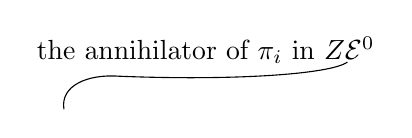
\begin{tikzpicture}[x=1cm,y=1cm]\node at (0,.35) {the annihilator of $\pi_i$ in $\mathfrak Z\mathcal E^0$};\draw (-1.8,-.4) .. controls (-1.85,-.1) and (-1.5,.05) .. (-1.1,.02) .. controls (.4,-.04) and (1.6,.05) .. (1.8,.2);\end{tikzpicture}}} is the ideal of the $u\in\mathfrak Z\mathcal E^0$ such that $\mathcal E_i^{2n-i}u=0$; now in a commutative ring, an idempotent is known when one knows its annihilator. Likewise for $\pi_{2n-i}$, its annihilator in $\mathfrak Z\mathcal E^0$ consists of the $u\in\mathfrak Z\mathcal E^0$ such that $u\mathcal E_i^{2n-i}=0$.

At the same time, the conditions $(3.1.)_i$, $(3.2.)_i$ for every $i$, give a \deleted{condition} procedure for determining the $\pi_i$ step by step.

\figure{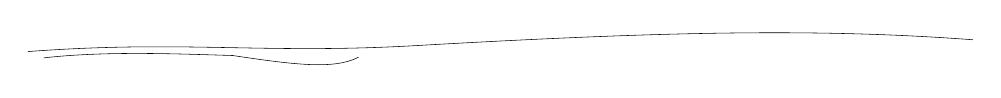
\begin{tikzpicture}[x=1cm,y=1cm]\draw[line width=.2pt] (0,0) .. controls (2,.15) and (3,-.04) .. (5,.08) .. controls (8,.25) and (10,.30) .. (12,.15);\draw[line width=.2pt] (.2,-.08) .. controls (1,.01) and (1.9,-.03) .. (2.6,-.05) .. controls (3.4,-.17) and (3.9,-.23) .. (4.2,-.07);\end{tikzpicture}}

4. When $\mathcal E^*$ is as in 1., a sufficient condition for having $(3.1)_i$ \inserted{or v. $(3.2)_i$} is the \deleted{sufficient} following

$(4.1)_i$ The intersection of the kernels of the $\unsure{v|u}:M^i\longrightarrow M^{2n-i}$, for $v\in\mathcal E_i^{2n-i}$, is reduced to $0$.

$(4.2)_i$ The sum of the images of the $v:M^i\longrightarrow M^{2n-i}$, for $v\in\mathcal E_i^{2n-i}$, is \deleted{\unsure{to}} equal to $M^{2n-i}$.

These two conditions are satisfied if one has

$(4.3)_i$ There exists \inserted{\figure{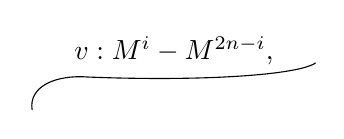
\begin{tikzpicture}[x=1cm,y=1cm]\node at (0,.35) {$v:M^i-M^{2n-i}$,};\draw (-1.8,-.4) .. controls (-1.85,-.1) and (-1.5,.05) .. (-1.1,.02) .. controls (.4,-.04) and (1.6,.05) .. (1.8,.2);\end{tikzpicture}}} $v\in\mathcal E_i^{2n-i}$, which is an isomorphism from
\mspage{5}
